\documentclass[11pt,a4paper]{article}
\usepackage[margin=.85in]{geometry}
\usepackage[T1]{fontenc}\usepackage{lmodern,microtype,amsmath,amssymb,amsthm,graphicx,booktabs,tikz,enumitem,placeins}
\usetikzlibrary{positioning,arrows.meta}
\usepackage[colorlinks=true,linkcolor=blue!45!black,urlcolor=blue!45!black,citecolor=blue!45!black]{hyperref}
\pagestyle{empty}
\setcounter{secnumdepth}{0}
\setcounter{tocdepth}{3}
\setlength{\parindent}{0pt}\setlength{\parskip}{5pt}\setlength{\abovedisplayskip}{8pt}\setlength{\belowdisplayskip}{8pt}
\newcommand{\E}{\mathbb E}
\newcounter{studyfig}
\makeatletter
\setlength{\@fptop}{0pt}
\setlength{\@fpsep}{16pt}
\setlength{\@fpbot}{0pt plus 1fil}
\makeatother
\hypersetup{pdftitle={COBRA: Condorcet-Or-Borda Reuse Algorithm},pdfauthor={Pranav Bhatnagar and Praveen Kumar S}}
\begin{document}
\hypersetup{pageanchor=false}\begin{titlepage}\thispagestyle{empty}\centering\vspace*{1.3cm}
{\Large Learning from Human Preferences\par}\vspace{1.2cm}
{\Huge\bfseries COBRA\par}\vspace{.4cm}
{\LARGE Condorcet-Or-Borda Reuse Algorithm\par}\vspace{.7cm}
{\Large Reusing diagnostic comparisons while preserving\\ logarithmic finite-horizon regret\par}\vspace{1.4cm}
{\large Project report based on Zoghi et al. (2014)\par}\vspace{1cm}
\begin{tabular}{ll}\toprule\textbf{Team member}&\textbf{Roll number}\\\midrule Pranav Bhatnagar&ED23B037\\Praveen Kumar S&ED23B038\\\bottomrule\end{tabular}
\vfill
\begin{minipage}{.87\linewidth}\textbf{Central question.} Once a Condorcet winner has been ruled out, can its diagnostic comparisons help identify a Borda winner with fewer additional duels? We combine a finite-horizon correctness and regret argument with paired synthetic and empirical-preference simulations.\end{minipage}
\vfill\end{titlepage}
\pagenumbering{roman}\hypersetup{pageanchor=true}\thispagestyle{empty}\tableofcontents\clearpage\pagenumbering{arabic}
\section{Introduction: a winner assumption worth checking}

Pairwise feedback is often easier to obtain than an absolute score. A user can choose between two recommendation lists without assigning either a numerical utility. A judge can compare two performances, and an election ballot can express which candidate is preferred. In a dueling bandit problem the learner repeatedly selects a pair, observes its winner, and seeks a good alternative while limiting the cost of exploration.

Relative Upper Confidence Bound (RUCB) is our starting point \cite{rucb}. Its central structural assumption is the existence of a \emph{strict Condorcet winner}: an arm that beats every other arm with probability greater than one half. RUCB maintains optimistic pairwise estimates, chooses a potential champion, and tests it against an optimistic challenger. Under its assumptions, the leading time-dependent regret term is logarithmic. The assumption is weaker than a complete transitive ranking, but is not guaranteed by the presence of individually transitive voters.

Our project asks one question: \textbf{after comparisons have ruled out a Condorcet winner, can those observations reduce the additional duels needed to identify a Borda winner?} We retain a Condorcet-first objective: if a strict Condorcet winner exists, it is preferred; otherwise the target is the alternative with greatest mean winning probability against a uniformly random opponent. This priority is our decision rule, not a universal welfare claim.

The question is motivated by cyclic majority preferences. Different voters may favor different alternatives strongly enough that the majority prefers $A$ to $B$, $B$ to $C$, and $C$ to $A$. This is a cycle, rather than a ``cyclic winner.'' Cycles can occur in a small part of a larger preference matrix even while another alternative beats everybody. Thus observing a cycle is not itself a certificate of Condorcet non-existence.

We study two empirical ranking collections from PrefLib: figure-skating judges and Electoral Reform Society (ERS) elections \cite{preflib,skate,ers}. Their audited matrices contain cycles. We explicitly distinguish full profiles from cycle-induced subsets. The latter provide real-preference fallback instances, but are selected stress tests rather than representative random samples.

Our contribution is a reproducible empirical investigation, supported by a finite-horizon correctness and regret argument. Condorcet testification and the Borda reduction are established ingredients \cite{test,sparse}. We compare paired runs that share diagnosis and future random samples, differing only in whether diagnostic evidence may accelerate fallback certification. We also examine when conservative confidence bounds prevent useful reuse. The theorem preserves linear explicit dependence on $K$ and logarithmic dependence on $T$ under stronger separation assumptions; it is not a new proof of RUCB's original anytime result.

\section{Definitions and the cyclic counterexample}

Let $[K]=\{1,\ldots,K\}$, $K\ge2$. For distinct arms, $p_{ij}$ is the probability that $i$ wins against $j$. We assume $p_{ji}=1-p_{ij}$, set $p_{ii}=1/2$, and write $P=(p_{ij})$. Each queried pair produces a fresh independent Bernoulli observation with this fixed mean. Independence refers to the simulator's sampling model; a finite survey does not establish population independence or stationarity.

A strict Condorcet winner $c$ satisfies $p_{cj}>1/2$ for all $j\ne c$; it is unique if it exists. The Borda score and winner are
\[
b_i=\frac{1}{K-1}\sum_{j\ne i}p_{ij},\qquad b^\star\in\arg\max_i b_i.
\]
A maximizer always exists in a finite set, but uniqueness requires a positive Borda gap $\Delta_B=\min_{i\ne b^\star}(b_{b^\star}-b_i)$.

Consider the valid reciprocal matrix
\[
P=\begin{pmatrix}.50&.60&.35\\.40&.50&.70\\.65&.30&.50\end{pmatrix},
\qquad (b_A,b_B,b_C)=(.475,.550,.475).
\]
Every arm has a strict loss, yet $B$ has the largest Borda score. The matrix can be generated by a distribution of strict rankings: $30\%$ rank $A>B>C$, $35\%$ rank $B>C>A$, $30\%$ rank $C>A>B$, and $5\%$ rank $B>A>C$. Thus the example does not require individual voters to be inconsistent.

RUCB's optimistic candidate set is $C_t=\{i:u_{ij}(t)\ge1/2\ \forall j\}$. In this matrix, no row of the true matrix satisfies that requirement. This does not imply that finite-sample $C_t$ must become permanently empty: confidence bonuses can revive candidates. It means that the original winner assumption and its associated regret analysis cannot simply be applied.

Replacing only the returned arm is also insufficient. If $B$ is chosen as champion, RUCB's challenger rule can select $A$, since $p_{AB}=.60$. Continued $B$--$A$ comparisons incur positive Borda regret. Finding a Borda target requires learning average performance, not merely treating its strongest opponent as the benchmark.

We define the hierarchical target as the Condorcet winner if present and the unique Borda winner otherwise. The two winners may disagree even when a Condorcet winner exists. This is why we do not evaluate a Condorcet-first algorithm using Borda regret on every matrix.

Exact ties are a separate boundary issue: absence of a \emph{strict} Condorcet winner does not necessarily mean every arm has a strict loss. An arm can tie another and lose to none. Our clean theorem excludes pairwise ties, and budget exhaustion is always reported as inconclusive rather than as evidence of a cycle.

\section{Proposed procedure and relationship to prior work}

The method is a finite-horizon, diagnose-then-fallback construction inspired by RUCB. It replaces RUCB's champion--challenger schedule rather than inheriting its proof unchanged. Testification asks whether a Condorcet winner exists and identifies it when it does; Haddenhorst et al. study this task and provide Noisy Tournament Sampling (NTS) \cite{test}. We implement the simpler select-then-verify construction, not NTS. Uniform-opponent Borda learning is an established reduction \cite{sparse}; Borda-Confidence-Bound provides a related logarithmic-regret reference \cite{bcb}.

\begin{center}
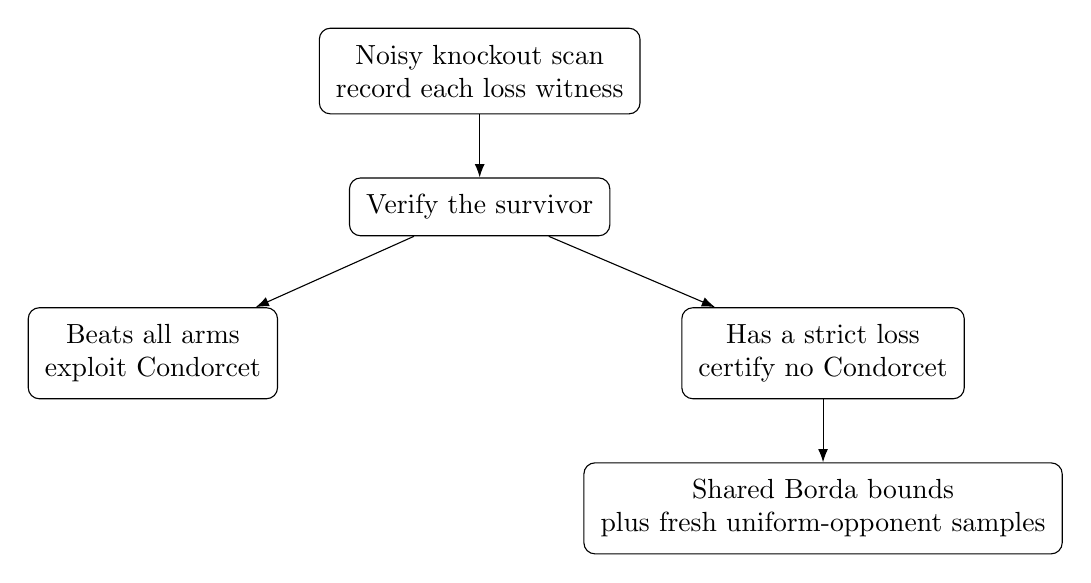
\begin{tikzpicture}[node distance=8mm,box/.style={draw,rounded corners,align=center,inner sep=6pt},>=Latex]
\node[box] (a) {Noisy knockout scan\\record each loss witness};
\node[box,below=of a] (b) {Verify the survivor};
\node[box,below left=9mm and 9mm of b] (c) {Beats all arms\\exploit Condorcet};
\node[box,below right=9mm and 9mm of b] (d) {Has a strict loss\\certify no Condorcet};
\node[box,below=of d] (e) {Shared Borda bounds\\plus fresh uniform-opponent samples};
\draw[->] (a)--(b);\draw[->](b)--(c);\draw[->](b)--(d);\draw[->](d)--(e);
\end{tikzpicture}
\end{center}
\textbf{Sampling and storage.} Let $W_{ij}$ count wins and $N_{ij}=W_{ij}+W_{ji}$ count duels. Every observation updates the same pairwise matrix. Diagnostic block outcomes are stored separately from statistical matrix intervals: a fixed-block majority decision and an interval excluding $1/2$ are different events.

\textbf{Diagnosis.} Scan arms in a fixed order. Retain the estimated winner of each comparison and record the other's loss. Then test the survivor against all remaining arms. If it beats everyone, return it. If it loses once, every arm now has a loss witness and no Condorcet winner exists. Previously resolved pair tests may be cached.

\textbf{Fallback.} Both policies receive the same fresh uniform-opponent samples and inspect the same direct Borda stopping condition at the same checkpoints. Restart uses only direct score intervals. Reuse also uses row-average intervals from the shared pairwise matrix and intersects the two sets of valid intervals. It can stop early if this extra evidence separates a winner. It does not change future samples or eliminate pairwise losers from Borda consideration.

\textbf{Exploitation and budgets.} Once a target is identified, compare it against itself for the rest of the horizon. If time runs out before identification, output inconclusive; never infer non-existence from a timeout. Conservative finite sample caps make the theoretical exploration budget explicit. Our experimental checkpoints aggregate iid samples in batches; they do not create fractional duels.

\section{Correctness and regret analysis}
\subsection{A. Condorcet diagnosis}

\textbf{Assumptions for the guarantee.} The horizon $T$ is known; probabilities are stationary and reciprocal; every duel is fresh and independent; self-comparisons are allowed. A supplied constant $h>0$ satisfies $|p_{ij}-1/2|\ge h$ for all distinct pairs. Thus all pair directions exist. For exact fallback identification assume a unique Borda winner and a supplied lower gap bound $\Delta_0>0$. These are stronger promises than original RUCB requires. Experimental gap inputs are oracle-informed, as discussed in the experimental setup.

Fix total failure budget $\delta$ and split it into $d=\delta/3$ for each of diagnostic tests, matrix intervals and direct score intervals. For a requested unresolved pair use
\[
n_D=\left\lceil\frac{1}{2h^2}\log\frac{4K}{d}\right\rceil
\]
fresh duels and return its empirical majority direction. Empirical ties are broken by the specified implementation rule (the second queried arm). Conditional on the history before the block, a wrong direction requires an estimation error at least $h$. Hoeffding therefore gives
\[
\Pr(\text{wrong block decision}\mid\mathcal H)
\le2\exp(-2n_Dh^2)\le\frac{d}{2K}.
\]
\textbf{Lemma 1 (diagnostic soundness).} With probability at least $1-d$, every decision used by the knockout and verification procedure is correct, and its returned diagnosis is correct.

\emph{Proof.} There are $K-1$ knockout decisions. On their joint correctness event, each eliminated arm has an opponent that truly beats it. The witness need not survive the knockout. Since a genuine Condorcet winner loses no pair, it cannot be eliminated. Thus, if it exists, it is the final survivor.

Verification needs at most $K-1$ further decisions. If the survivor wins all of them it beats every arm and is Condorcet. If it loses, it too has a strict loss. Together with the earlier witnesses, every arm has a loss and none is Condorcet. This reasoning uses no transitivity.

There are fewer than $2K$ requested tests. A union bound over the conditional error probabilities gives failure at most $d$. Cached directions are outcomes of previously counted tests, so reusing them adds no new test error. The number of physical duels is at most $2(K-1)n_D$. \hfill$\square$

\textbf{What the lemma does not say.} It does not assert that our separate pairwise confidence interval excludes $1/2$ after $n_D$ observations. The block size is justified by the known separation and the majority error calculation. We use these block decisions for diagnosis and the time-uniform intervals on the next page for Borda reuse. This separation keeps the proof faithful to the code.

The implementation is also tested independently of randomness on all $2^{\binom42}=64$ strict four-arm tournaments. In each, deterministic knockout plus verification agrees with direct inspection of the matrix. These checks support the implementation; the argument above supplies general correctness.

\subsection{B. Safe reuse of pairwise observations}

Diagnostic sampling is highly nonuniform. An arm may be compared mainly with its difficult opponent. Consequently $\sum_jW_{ij}/\sum_jN_{ij}$ is not generally an estimate of its uniform-opponent Borda score. Reuse must preserve pair identity.

Let $M=\binom K2$. At pair sample count $n\ge1$, define
\[
r_P(n)=\sqrt{\frac{\log(4Mn^2/d)}{2n}},\quad
L_{ij}=\max\{0,\widehat p_{ij}-r_P(n)\},\quad
U_{ij}=\min\{1,\widehat p_{ij}+r_P(n)\}.
\]
For unsampled pairs use $[0,1]$; for self-pairs use $[1/2,1/2]$. Reverse intervals satisfy $L_{ji}=1-U_{ij}$ and $U_{ji}=1-L_{ij}$.

\textbf{Lemma 2 (simultaneous matrix coverage).} With probability at least $1-d$, every pair interval contains its true probability at every observation time, even when the pair selection is adaptive.

\emph{Proof.} Imagine an infinite iid outcome stream for each unordered pair, revealed sequentially when that pair is queried. At a fixed sample count Hoeffding gives
\[
\Pr\{|\widehat p_{ij}(n)-p_{ij}|>r_P(n)\}
\le2e^{-2nr_P(n)^2}=\frac{d}{2Mn^2}.
\]
A union bound over all unordered pairs and positive sample counts gives
\[
\Pr(\exists\,\text{failed interval})
\le M\sum_{n=1}^\infty\frac{d}{2Mn^2}
=\frac{\pi^2}{12}d<d.
\]
Since the event covers every sample count, it covers counts reached at adaptive stopping times. We have not conditioned a fixed-$n$ bound on a random count. \hfill$\square$

On this event the Borda row bounds
\[
B_i^- =\frac{\sum_{j\ne i}L_{ij}}{K-1},\qquad
B_i^+ =\frac{\sum_{j\ne i}U_{ij}}{K-1}
\]
contain $b_i$. Hence $B_a^->\max_{i\ne a}B_i^+$ certifies a unique Borda winner. All original arms remain in this check, including those eliminated during diagnosis. Removing pairwise losers would change the optimization problem and could remove the correct Borda winner.

When fresh direct score intervals are available, reuse intersects them with the matrix intervals:
\[
[A_i^-,A_i^+]=[\max(B_i^-,D_i^-),\min(B_i^+,D_i^+)].
\]
On simultaneous coverage this intersection is valid. A direct certificate is also a certificate of the intersection, so adding reuse cannot delay certification along the coupled sample path. If intersections are inconsistent off the good event, the optional acceleration is ignored and the direct procedure continues; such paths remain within the allocated failure event.

This pathwise dominance is a design property, not the empirical discovery. The experiments quantify its magnitude and how the distribution of diagnostic information affects the savings.

\subsection{C. Borda identification and comparison cap}

For a designated arm $i$, independently draw $J$ uniformly from $[K]\setminus\{i\}$. If $Y=\mathbf1\{i\text{ wins against }J\}$, then
\[
\E[Y\mid i,\mathcal H]=\frac1{K-1}\sum_{j\ne i}p_{ij}=b_i.
\]
The designated outcomes for that arm therefore form a Bernoulli score stream. The opponent's complementary outcome is not automatically a direct uniform-opponent sample for that opponent. It is stored in the pairwise matrix, but only designated samples update direct score estimates. This is the Borda reduction of Jamieson et al.\ \cite{sparse}.

With $m_i$ designated samples, use the time-uniform radius
\[
r_B(m)=\sqrt{\frac{\log(4Km^2/d)}{2m}},\qquad
D_i^- =\max(0,\widehat b_i-r_B(m_i)),\quad
D_i^+ =\min(1,\widehat b_i+r_B(m_i)).
\]
Unsampled direct intervals are $[0,1]$. The proof of Lemma 2, replacing $M$ by $K$, shows simultaneous direct coverage with failure less than $d$. This permits repeated checking without treating a fixed-count bound as a sequential one.

\textbf{Lemma 3 (Borda completion).} Let $\Delta_B\ge\Delta_0>0$. Let $n_{\rm cap}$ be the first power of two for which $r_B(n_{\rm cap})\le\Delta_0/8$. Sampling a least-observed designated arm until each has this many samples guarantees correct direct certification on the score-coverage event, within $Kn_{\rm cap}$ duels.

\emph{Proof.} At completion, for the true Borda winner $b$ and each other $i$,
\[
D_b^-\ge b_b-2r_B(n_{\rm cap}),\qquad
D_i^+\le b_i+2r_B(n_{\rm cap}).
\]
Thus
\[
D_b^- -D_i^+\ge \Delta_B-4r_B(n_{\rm cap})
\ge\Delta_0/2>0.
\]
The strict stopping condition must hold. Shared-data intersections can stop earlier, but use the same cap and future samples. \hfill$\square$

For an explicit sufficient value put $L=\log(64K/(d\Delta_0^2))$ and $m_0=\lceil256L/\Delta_0^2\rceil$, taking $0<\Delta_0\le1$. Then $m_0\le257L/\Delta_0^2$ and
\[
\log(4Km_0^2/d)\le2L+2\log257+2\log L\le8L.
\]
Here $L\ge\log128$, $2\log257\le3L$, and $2\log L\le2L$. Thus $r_B(m_0)^2\le\Delta_0^2/64$. The radius decreases for $m\ge1$, since $\log(4Km^2/d)>2$. Rounding to the next power of two gives $n_{\rm cap}<2m_0$. Consequently
\[
n_{\rm cap}=O\!\left(\Delta_0^{-2}\log\frac{K}{d\Delta_0}\right).
\]
Unlike a fixed-count majority construction, this version matches the experiment's sequential direct stopping rule. It adds a mild gap-dependent logarithm, which must remain visible before asymptotic simplification. The cap is a sufficient bound, not a prediction of actual stopping time.

For Borda-only explore-then-commit learning, the same argument immediately gives logarithmic time dependence when $d$ is calibrated to $T$. Related logarithmic Borda regret is already established in BCB's fixed-gap setting \cite{bcb}; our analysis is an explicitly stationary composition, not a claim to originate that result.

\subsection{D. Combined regret guarantee}

Our performance criterion follows the selected priority rule. On a Condorcet instance with winner $c$, put $\Delta_i^C=p_{ci}-1/2$ and
\[
r_t=\tfrac12(\Delta_{I_t}^C+\Delta_{J_t}^C).
\]
Otherwise use $r_t=b_b-(b_{I_t}+b_{J_t})/2$, where $b$ is the unique Borda winner. In both cases $0\le r_t\le1$, and choosing the correct target against itself has zero regret. Write $R_T=\sum_{t=1}^T r_t$.

\textbf{Theorem 1 (finite-horizon composition).} Under the stated model and separation promises, use total error budget $\delta=T^{-2}$ and $d=1/(3T^2)$. Let
\[
N_0=2(K-1)n_D+Kn_{\rm cap}.
\]
For either policy, including the reuse acceleration,
\[
\Pr\{R_T\le\min(T,N_0)\}\ge1-T^{-2},\qquad
\E R_T\le\min(T,N_0)+T^{-1}.
\]

\emph{Proof.} Lemmas 1--3 supply three events, each failing with probability at most $d$. Their intersection therefore has probability at least $1-3d$. If diagnosis returns a Condorcet winner it is the correct target. If it returns no-CW, direct Borda identification or an earlier valid shared-data certificate returns the correct fallback. The latter coverage event is valid for adaptively collected observations. Fresh score coverage can be viewed conditionally on entering fallback, or through pre-generated independent score streams.

On this good event exploration takes at most $N_0$ duels and correct exploitation has zero regret. Truncating at the horizon bounds exploration by $\min(T,N_0)$. On the failure event, all additional exploitation regret is at most $T$. Hence $\E R_T\le\min(T,N_0)+T(3d)$, proving the claims. \hfill$\square$

Substituting the diagnostic block size and Borda cap gives
\[
\E R_T=O\!\left[
\frac K{h^2}\log(KT)
+\frac K{\Delta_0^2}\log\frac{KT}{\Delta_0}+K\right].
\]
For fixed positive $h,\Delta_0$ and $T\ge K$, this is $O(K\log T)$. The diagnostic and fallback costs \emph{add}; we do not multiply their sample counts. This is a regret bound over a $T$-round run, not a claim that the run contains only $O(K\log T)$ iterations.

The bound is conservative: it charges every exploratory duel one unit, ignores instance-dependent loss costs, and uses a uniform worst-pair separation. It is not a proof that $O(K\log T)$ is the best achievable bound in every subclass. It also does not match RUCB's original gap constants or provide a horizonless all-time guarantee. If margins shrink with $K$ or $T$, their factors cannot be hidden. A fixed-confidence choice such as $\delta=.05$ gives a possible $\delta T$ expected exploitation term and is not covered by the logarithmic expected-regret claim.

\section{Experiments}
\subsection{Experimental setup}

Experiment A measures additional-duel savings, B varies difficulty, C evaluates regret and Condorcet priority, and D compares sufficient budgets with observed costs. Separate implementations apply the method to figure-skating rankings and ERS election ballots. All numerical results come from the recorded simulation runs.

\textbf{Paired control.} For a seed and matrix, both methods share the complete diagnosis, its observations, arm order, fresh opponent draws and duel outcomes. We simulate the fresh stream until Restart stops and record when Reuse would have stopped on its prefix. Direct stopping rules, caps and checkpoints are identical. Reuse alone may intersect shared-matrix intervals with direct score intervals. Savings therefore measure an information-reuse stopping option, not a comparison against a baseline forced to exhaust its cap.

\textbf{Confidence and oracle inputs.} A, B and the real-data identification tests use total error budget $.05$, split into three equal parts. C uses $T^{-2}$ to match Theorem 1. For controlled simulation we supply $h=.8\min_{i<j}|p_{ij}-.5|$ and $\Delta_0=\Delta_B$ from the simulator matrix. The learner does not use its unknown probabilities to choose the target, but these oracle-informed tuning values are strong side information. A practical implementation would need supplied lower bounds or a separate unknown-gap analysis. All comparisons use the same inputs, so the paired reuse contrast is fair within this setting.

\textbf{Batching.} Fallback samples are taken in blocks of 2048 designated duels (256 in C), assigning opponents by a multinomial draw and outcomes by independent binomials. These are exact aggregates of iid duels. Certificates are inspected at block boundaries, so stopping times can exceed per-duel checking by a checkpoint delay. The same delay applies to both policies. Caps are enforced without overshooting; completed least-observed streams differ by at most one block.

\textbf{Replication.} A and each real subset use 60 seeds, B uses 30 seeds per parameter cell, and C uses 20 seeds per horizon and hybrid policy. RUCB is run with $\alpha=.51$ for eight seeds through 300,000 rounds, recording its horizonless trajectory at the same horizons. It follows the paper's candidate, remembered-champion and challenger rules, with unsampled off-diagonal indices set to 2 under its $x/0=1$ convention for both terms. We use RUCB as a behavioral reference, not as a confidence-correct stopping baseline.

\textbf{Uncertainty and censoring.} Error bars are mean $\pm1.96$ standard errors across independent seeded runs, not simultaneous confidence bands or population-survey uncertainty. Every attempted run remains in the recorded denominator. A horizon-truncated run is inconclusive and still incurs its observed regret. Zero observed errors do not establish zero error probability. For $n$ independent error-free trials, the one-sided 95\% binomial upper bound is $1-.05^{1/n}$.

The two real cases are empirical-matrix simulations: each duel is a fresh Bernoulli draw using the observed profile's pairwise fraction. They are not held-out predictions about unseen voters. Candidate subset selection is deterministic and outcome-independent with respect to simulated algorithm performance, but intentionally selects cyclic stress cases; prevalence claims are therefore excluded.

\subsection{A. Additional duels after diagnosis}

We begin with a separated three-cycle and a near-boundary cycle. The former uses the motivating matrix. The latter sets $p_{AB}=.55$, $p_{BC}=.75$, $p_{CA}=.51$: every arm loses somewhere, but the $C$--$A$ direction is difficult to establish. Borda scores are $(.52,.60,.38)$, so the Borda winner remains well separated even though diagnosis becomes harder.

Both methods first perform the same diagnosis and then see the same fresh Borda stream. The diagnostic count is not credited as a saving: it is common to both and is reported separately. The table includes all 60 runs per case.
\begin{center}\begin{tabular}{lrrrr}\toprule
Case & Diagnosis & Restart extra & Reuse extra & Saving\\\midrule
Cycle & 1,545 & 29,628 & 25,771 & 13.0\% \\
Near boundary & 154,203 & 22,801 & 0 & 100.0\% \\
\bottomrule\end{tabular}\end{center}
    \begin{figure}[htbp]\centering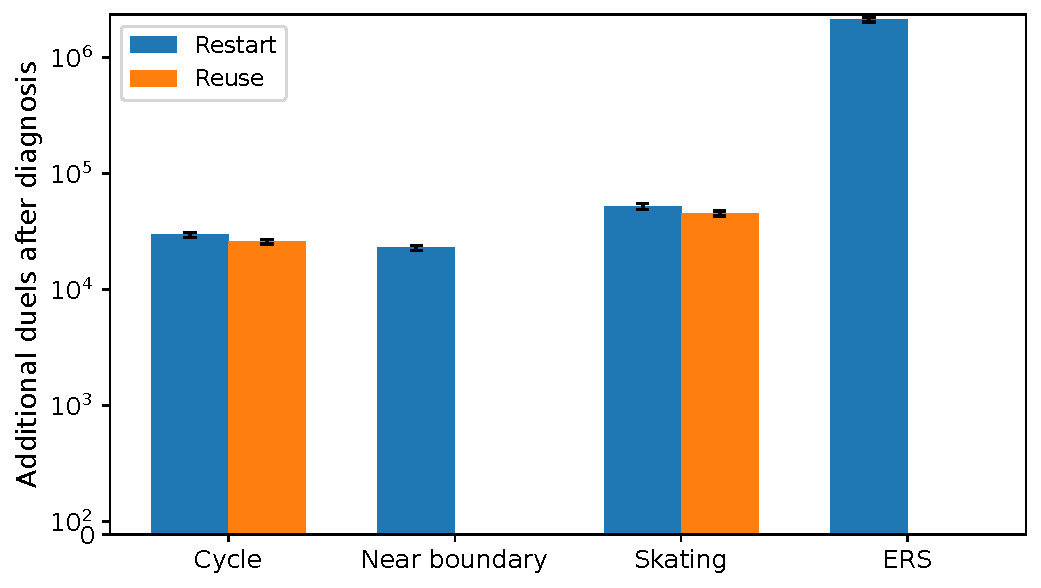
\includegraphics[width=.94\linewidth]{figures/additional_duels.pdf}
\caption{Mean additional duels, with 95\% normal-approximation error bars. The vertical axis is logarithmic above 1,000 and linear below it, including zero. The real cases are described in the implementation sections. Diagnosis is excluded here but included in total cost and regret.}\end{figure}


The comparison asks how much of the work already paid for during diagnosis can help the next task. Matrix reuse can certify immediately if the diagnostic observations have already narrowed all relevant Borda rows. Otherwise it intersects those bounds with the gradually improving direct bounds. The guarantee does not promise a positive saving on every run.

The near-boundary case must be interpreted carefully. Our fixed block size uses the smallest pairwise separation for \emph{every} diagnostic pair. A single hard edge therefore increases sampling on the easier diagnostic edges too. Any large reuse advantage partly recovers the cost of that conservative diagnosis. It should not be presented as evidence that this diagnosis is the most efficient available method.

\subsection{B. Sensitivity to preference gaps}

We vary the same three-arm template, keeping $p_{AB}=.55$ while choosing $p_{CA}\in\{.51,.53,.57,.65\}$ and $p_{BC}\in\{.68,.75,.85\}$. All tested matrices are no-CW cycles. The pairwise diagnostic separation and Borda gap are computed and recorded for each cell; one is not assumed to be a proxy for the other. Cases with a Borda gap below $.005$ are excluded by the declared generator rule, not after inspecting performance.

There are 30 paired seeds per retained cell. The plotted statistic is the mean of the \emph{per-run} fractional savings, $100(N_{\rm restart}-N_{\rm reuse})/N_{\rm restart}$, with a standard-error interval. This differs from the ratio of the two means used in the preceding table.
\begin{figure}[htbp]\centering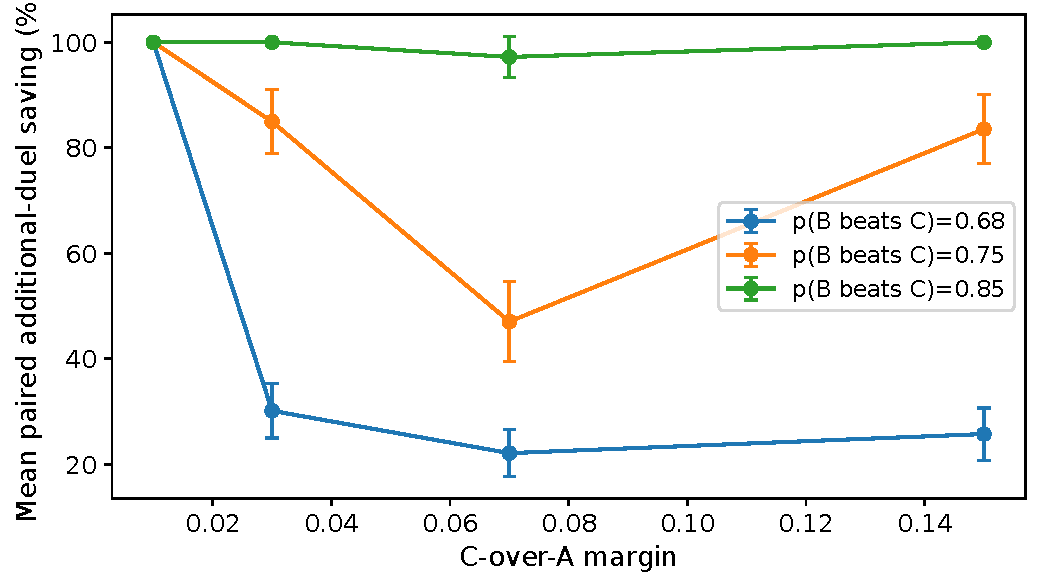
\includegraphics[width=.94\linewidth]{figures/sensitivity.pdf}
\caption{Sensitivity to the C-over-A margin, for three strengths of B-over-C preference. Both diagnosis and Borda difficulty change across the grid; the figure measures their combined effect, not a one-variable causal estimate.}\end{figure}


Across retained cells, the ratio-of-means savings ranged from 22.2\% to 100.0\%. These are measured descriptive ranges, not a theorem about all preference matrices.

Reuse should be most useful when the diagnostic sample allocation covers the comparisons needed to separate the leading Borda scores. A candidate can be disqualified from Condorcet status by one comparison, while its Borda score depends on its whole row. This explains why a certificate of no-CW can coexist with wide Borda intervals.

The uniform-opponent direct estimator aggregates information more efficiently than conservative row intervals in some regimes. Merely storing more pair counts does not guarantee useful reuse. Our intersection rule preserves the direct estimator as a safe alternative, so unhelpful matrix bounds should yield little or no saving rather than slower fresh-sample stopping.

\subsection{C. Regret on cyclic instances}

Theorem 1 concerns a family of horizon-calibrated runs. We therefore rerun diagnosis and fallback with $\delta=T^{-2}$ separately for $T\in\{10^4,3\cdot10^4,10^5,3\cdot10^5\}$. These hybrid points are not prefixes of a single anytime algorithm. Every diagnostic and fallback comparison contributes to the reported hierarchical regret; after certification the target is compared against itself.
\begin{figure}[htbp]\centering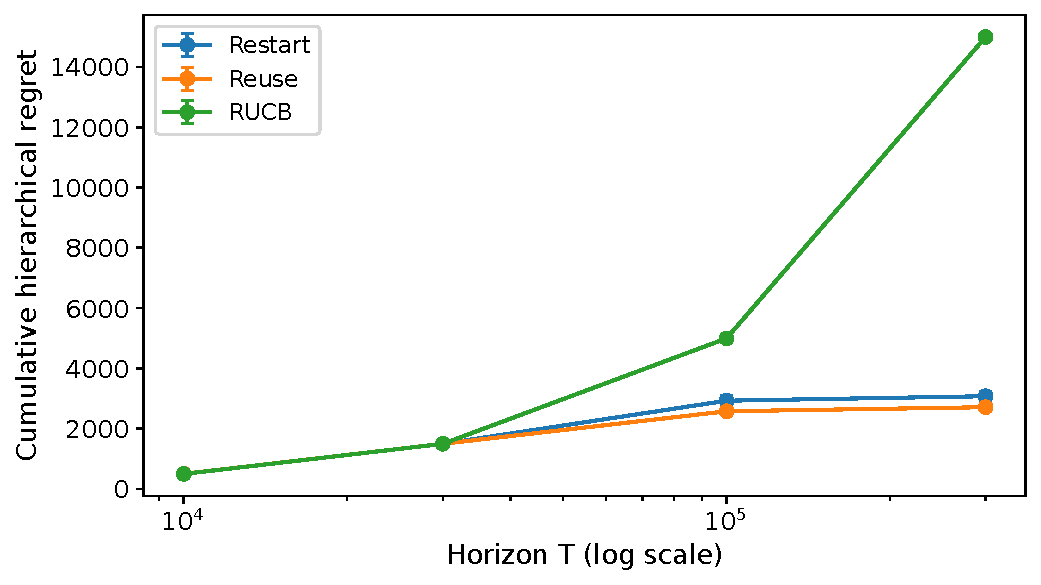
\includegraphics[width=.94\linewidth]{figures/regret_Cycle.pdf}
\caption{Cumulative Borda regret on the separated no-CW cycle; horizontal position is logarithmic in T. Hybrid means use 20 seeds per horizon; RUCB uses eight horizonless trajectories. Error bars describe seeded simulation variation.}\end{figure}


On this matrix the hierarchical objective is exactly Borda regret. Original RUCB has no true Condorcet target. Its strongest-challenger rule keeps sampling distinct arms: the existence of some arm beating each possible champion prevents the zero-regret Condorcet exploitation argument from applying. The plot is an empirical comparison under an intentionally violated assumption, not a contradiction of RUCB's theorem.

The finite-horizon hybrid must buy increasingly reliable evidence as $T$ grows. If horizons are too short, the plotted result is dominated by unfinished exploration. If enough budget is available, exploitation costs zero on the good event. The theorem supplies the logarithmic statement; four finite horizons can only check consistency with its predicted behavior and reveal startup effects.

We do not fit a line and claim to have established asymptotic complexity from a graph. We also do not hide the $h^{-2}$ and $\Delta_0^{-2}$ constants: for small margins they can dominate the entire practical horizon. The final discussion addresses this mismatch between a valid rate and an efficient method.

\subsubsection{Preserving Condorcet priority}

Two further instances test whether the method retains its intended objective. In the agreement case $p_{AB}=.70$, $p_{BC}=.65$, $p_{CA}=.30$; $A$ is both Condorcet and Borda winner. In the disagreement case $p_{AB}=.55$, $p_{BC}=.75$, $p_{CA}=.40$; $A$ is Condorcet but Borda scores are $(.575,.600,.325)$, so $B$ wins on average. The required output remains $A$.
\begin{figure}[htbp]\centering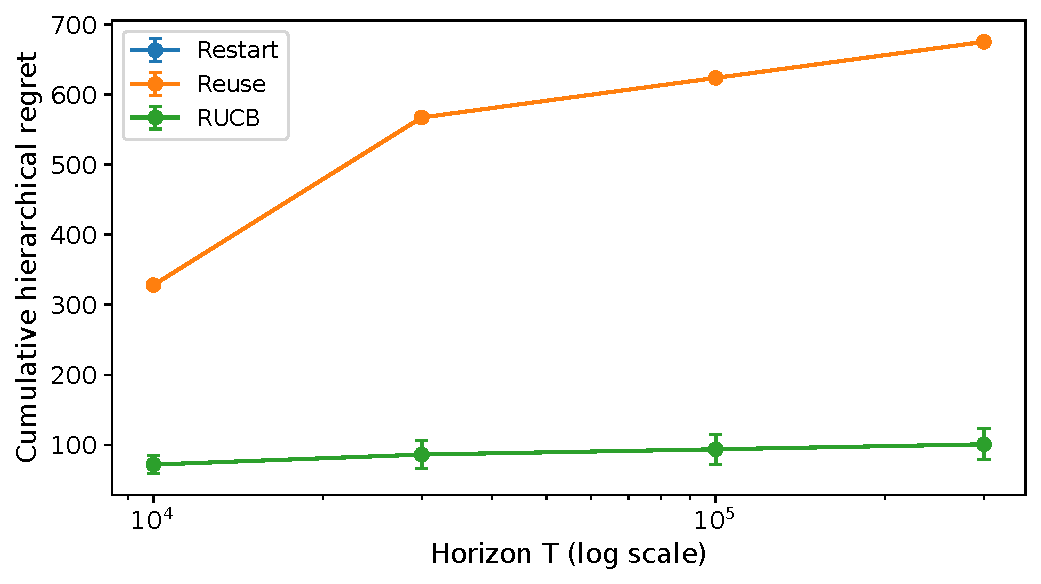
\includegraphics[width=.94\linewidth]{figures/regret_CW_disagreement.pdf}
\caption{Condorcet regret on the disagreement instance. A direct Borda learner would optimize a different target, so it is not treated as an interchangeable baseline here.}\end{figure}


On correctly diagnosed CW runs the Borda phase is never entered. Restart and Reuse consequently coincide along the paired path. Their comparison is a built-in control: a claimed reuse benefit on this branch would indicate an accounting error. RUCB has substantially lower regret than both hybrids on the tested CW controls: diagnosis is overhead when its assumption already holds.

The disagreement case is shown because it is more informative about our decision rule. The agreement case is retained as a control; the discussion reports its completion and regret outcomes.

The test does not prove that Condorcet should always have priority in an application. It checks faithful implementation of our explicitly chosen hierarchy. In recommendation, average performance might instead be the preferred objective, in which case direct Borda learning would avoid diagnosis altogether. The diagnostic cost is justified only when checking Condorcet existence serves the application.

\subsection{D. Sufficient comparison budgets}

The sufficient cap from Theorem 1 is intentionally distinct from measured stopping times. It guarantees a correct decision on the common confidence event under our supplied margins. It does not say that every run needs that many observations. The direct intervals and shared intervals are checked earlier, allowing both methods to stop before the cap.
\begin{figure}[htbp]\centering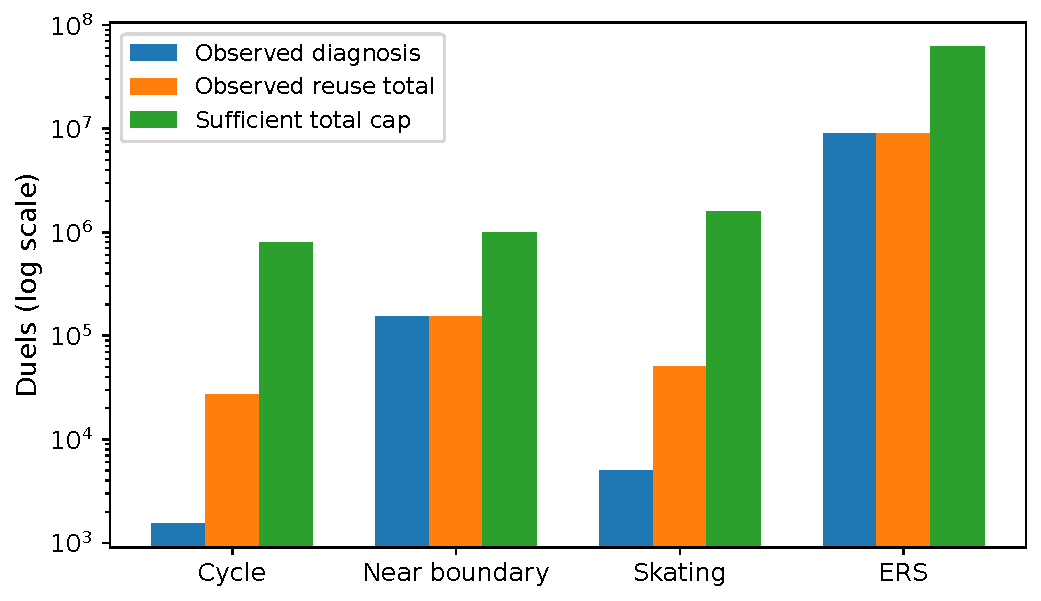
\includegraphics[width=.94\linewidth]{figures/sufficient_budgets.pdf}
\caption{Observed mean diagnosis, observed mean total Reuse duels, and the sufficient total exploration cap $2(K-1)n_D+Kn_{
m cap}$. The vertical axis is logarithmic because the ERS near-tie produces a much larger diagnostic cost.}\end{figure}


The figure includes diagnostic cost rather than crediting it as free evidence. When reuse saves nearly all fresh duels, the total procedure may still be expensive because those observations were purchased during diagnosis. On the ERS subset, a very small pairwise margin requires a large worst-pair block size even though the Borda gap is larger. This is a concrete limitation of our bounded baseline.

The cap is sufficient for the simulated empirical matrix under known lower bounds and independent binary feedback. It does not certify that the underlying population preferences equal that matrix. Nor is the cap a lower bound: sequential pair tests, instance-dependent tournament algorithms, or more efficient Borda procedures may need fewer samples. Our comparison isolates reuse within one transparent procedure.

For C, confidence is stricter and depends on each horizon, so those runs have different caps. If a cap exceeds $T$, the theorem still yields the valid but potentially uninformative bound $\E R_T\le T+1/T$. We retain horizon-truncated runs rather than asserting that every plotted horizon reaches the asymptotic regime.

The graph also highlights why regret and sample complexity must be kept separate. A long run can have low regret after correct exploitation. Our mathematical bound charges all exploratory comparisons at their maximum possible regret; the plotted regret uses the matrix-dependent loss of each selected pair.

\FloatBarrier\section{Implementation}
\subsection{Figure-skating judges' rankings}
We apply the method to judges ranking competitors in 1998 figure-skating competitions, from PrefLib \cite{skate}. The selected profile contains 9 voters and 24 alternatives. Its original identifier is \texttt{00006-00000028.soc}. The full profile has a strict Condorcet winner (original candidate ID 24). We do not claim that the complete profile is a no-Condorcet instance.

\textbf{Construction of the implementation case.} We scan files and candidate triples lexicographically and retain the first strict three-cycle with a unique Borda winner. Selection uses the preference profile, not the simulated performance of either method. This produces a disclosed cyclic stress test rather than an estimate of the prevalence of cycles. The retained original candidate IDs are 2, 5, 17, in that order. The observed pairwise matrix is
\[P=\begin{pmatrix}0.5000&0.6667&0.4444\\0.3333&0.5000&0.5556\\0.5556&0.4444&0.5000\end{pmatrix}.\]
The strict judge rankings yield a directed majority cycle on these three competitors, although the full competition retains a Condorcet winner. Sampling a pair uses the empirical fraction of judges preferring its row candidate.\par\begin{figure}[htbp]\centering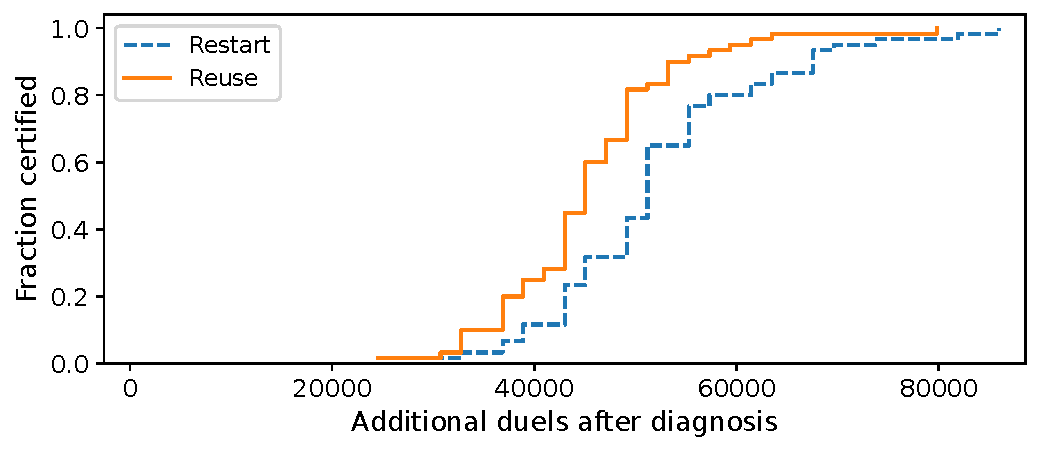
\includegraphics[width=0.88\linewidth]{figures/implementation_skating.pdf}
\caption{Figure-skating judges' rankings: additional duels needed for certification over 60 paired runs. Both methods share diagnosis and the fresh sample stream; Reuse has the additional shared-matrix stopping option. The curves include every run.}\end{figure}

\textbf{Results on this dataset.} Mean additional duels were 51,985 for Restart and 45,227 for Reuse, a 13.0\% reduction. The common diagnosis cost averaged 4,998 duels. All 60 runs per method completed with the correct Borda target at the identification confidence budget.

At horizon $T=300{,}000$, using the stricter horizon-calibrated budget, mean regret was 5,453 (Reuse), 6,641 (Restart), and 16,678 (RUCB), with 20/20 Reuse runs completing. The reduction in fresh sampling accompanies successful fallback in this case. These are simulations conditional on an empirical matrix, not new human trials or held-out population predictions. Small voter samples, the intentional candidate restriction, and any tied-completion choice limit generalization.\par
\FloatBarrier\subsection{Electoral Reform Society election ballots}
We apply the method to ranked election ballots collected by the Electoral Reform Society, from PrefLib \cite{ers}. The selected profile contains 380 voters and 10 alternatives. Its original identifier is \texttt{00007-00000001.soi}. The full profile has a strict Condorcet winner (original candidate ID 1). We do not claim that the complete profile is a no-Condorcet instance.

\textbf{Construction of the implementation case.} We scan files and candidate triples lexicographically and retain the first strict three-cycle with a unique Borda winner. Selection uses the preference profile, not the simulated performance of either method. This produces a disclosed cyclic stress test rather than an estimate of the prevalence of cycles. The retained original candidate IDs are 2, 4, 7, in that order. The observed pairwise matrix is
\[P=\begin{pmatrix}0.5000&0.4842&0.5066\\0.5158&0.5000&0.4987\\0.4934&0.5013&0.5000\end{pmatrix}.\]
ERS ballots can be incomplete. We place unranked candidates jointly last, following the documented tied-completion convention. Each voter tie contributes half a win in either direction. A simulated duel is then binary, equivalent to independently drawing a voter and fairly breaking a tied comparison. The audit also found full ERS Set 5 without a strict Condorcet winner, but with pairwise ties; that full profile falls outside our uniform-separation theorem.\par\begin{figure}[htbp]\centering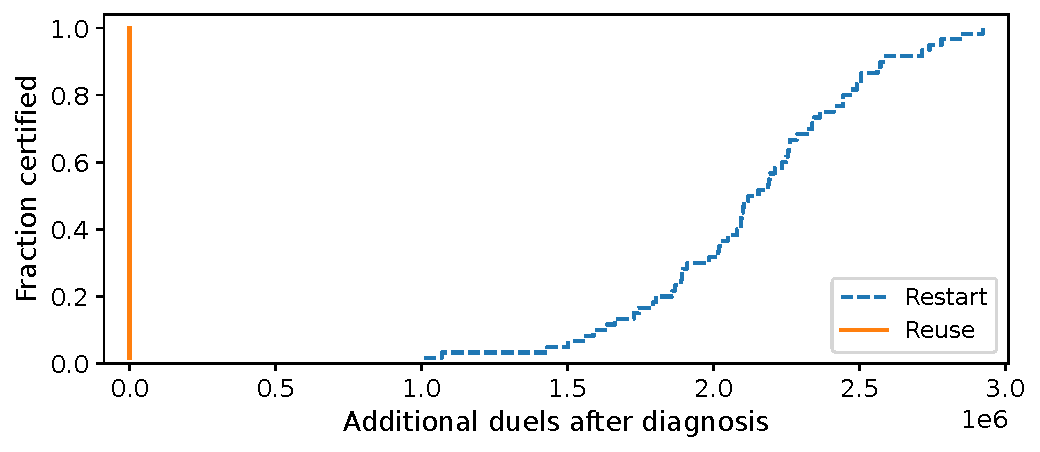
\includegraphics[width=0.88\linewidth]{figures/implementation_ers.pdf}
\caption{Electoral Reform Society election ballots: additional duels needed for certification over 60 paired runs. Both methods share diagnosis and the fresh sample stream; Reuse has the additional shared-matrix stopping option. The curves include every run.}\end{figure}

\textbf{Results on this dataset.} Mean additional duels were 2,125,005 for Restart and 0 for Reuse, a 100.0\% reduction. The common diagnosis cost averaged 8,906,664 duels. All 60 runs per method completed with the correct Borda target at the identification confidence budget.

At horizon $T=300{,}000$, using the stricter horizon-calibrated budget, mean regret was 1,776 (Reuse), 1,776 (Restart), and 2,120 (RUCB), with 0/20 Reuse runs completing. The hybrid diagnoses remained unfinished: lower observed regret here is not evidence of successful fallback. These are simulations conditional on an empirical matrix, not new human trials or held-out population predictions. Small voter samples, the intentional candidate restriction, and any tied-completion choice limit generalization.\par
\section{Results, reflection and limitations}

Across the synthetic identification tests and real-data implementations there were 1200 method-run records, with 0 incorrect completed answers and 0 inconclusive records. Because both policies share data, these records are paired, not independent samples for a two-method significance test. For a 60-seed error-free case, the one-sided 95\% upper bound on its true failure probability is still approximately 4.9\%, rather than zero.

The following finite-horizon outcomes include all runs. They help distinguish low regret due to successful exploitation from a horizon that ended before certification.
\begin{center}\begin{tabular}{lrrr}\toprule
Reuse case & $T$ & Completed & Mean regret\\\midrule
Cycle & 10,000 & 0/20 & 501 \\
Cycle & 300,000 & 20/20 & 2,712 \\
CW agreement & 10,000 & 20/20 & 153 \\
CW agreement & 300,000 & 20/20 & 200 \\
CW disagreement & 10,000 & 0/20 & 328 \\
CW disagreement & 300,000 & 20/20 & 675 \\
\bottomrule\end{tabular}\end{center}

\textbf{What we learned.} Condorcet diagnosis and Borda identification demand different evidence. A loss witness settles whether an arm can be Condorcet, but does not determine its average performance. Reuse is safe only when the estimator respects opponent allocation; the raw pooled win rate is not sufficient. The direct score intervals provide the essential escape from overly conservative matrix bounds.

\textbf{What remains limited.} We used known-margin, oracle-informed tuning and only three-arm cyclic stress tests. Our fixed-block diagnostic schedule over-samples easy comparisons when one pair is difficult. This can make reuse look more valuable by recovering work that a better diagnosis would avoid. Comparison with NTS and more efficient Borda identification is necessary before claiming state-of-the-art performance. The agreement control and completion checks support these conclusions; we present the most informative comparisons rather than grids of small plots.

The real matrices are estimated from small or finite voter populations; our repeated simulations quantify Bernoulli sampling variation conditional on those matrices. They do not quantify survey uncertainty. Selecting cyclic restrictions serves a stress-test objective and cannot estimate how often cycles occur in applications. ERS tied completion is a modeling choice, and ties or changing annotator behavior may violate the theorem's promises.

\textbf{Conclusion.} A finite-horizon Condorcet-first learner can diagnose failure, switch to a Borda target and preserve an $O(K\log T)$ regret order for fixed positive margins, with all diagnostic costs counted. Its shared observations can shorten fallback certification without changing the direct-sampling cap. The main empirical question is the size and conditions of that benefit, not whether concatenating two established algorithms is novel. Unknown gaps, unknown horizons, stronger baselines and held-out preference data are the natural next steps.

\textbf{AI assistance.} AI assisted with mathematical drafting, implementation and preparation of this report.

\FloatBarrier\clearpage\section{References}

\begingroup
\renewcommand{\section}[2]{}%
\begin{thebibliography}{9}
\bibitem{rucb} M. Zoghi, S. Whiteson, R. Munos, and M. de Rijke. Relative Upper Confidence Bound for the K-Armed Dueling Bandit Problem. \emph{ICML}, PMLR 32(2):10--18, 2014.\newline\url{https://proceedings.mlr.press/v32/zoghi14.html}
\bibitem{test} B. Haddenhorst, V. Bengs, J. Brandt, and E. H\"ullermeier. Testification of Condorcet Winners in Dueling Bandits. \emph{UAI}, PMLR 161:1195--1205, 2021.\newline\url{https://proceedings.mlr.press/v161/haddenhorst21a.html}
\bibitem{sparse} K. Jamieson, S. Katariya, A. Deshpande, and R. Nowak. Sparse Dueling Bandits. \emph{AISTATS}, PMLR 38:416--424, 2015.\newline\url{https://proceedings.mlr.press/v38/jamieson15.html}
\bibitem{bcb} A. Saha, T. Koren, and Y. Mansour. Adversarial Dueling Bandits. \emph{ICML}, PMLR 139:9235--9244, 2021. See Section 4, Borda-Confidence-Bound.\newline\url{https://proceedings.mlr.press/v139/saha21a.html}
\bibitem{preflib} N. Mattei and T. Walsh. PrefLib: A Library for Preferences. \emph{ADT}, 2013. Dataset archive and format specification:\newline\url{https://github.com/PrefLib/PrefLib-Data}
\bibitem{skate} PrefLib. Skate Data, collection 00006: 1998 figure-skating competition rankings. Selected file 00006-00000028.soc. Accessed 21 November 2026.\newline\url{https://preflib.github.io/PrefLib-Jekyll/dataset/00006}
\bibitem{ers} PrefLib. Electoral Reform Society Data, collection 00007. Selected file 00007-00000001.soi. Accessed 21 November 2026.\newline\url{https://preflib.github.io/PrefLib-Jekyll/dataset/00007}
\end{thebibliography}\endgroup

\subsection*{Project repository}\url{https://github.com/pranav1785/COBRA}
\end{document}
